\newpage

\subsection{Расчёт системы вентиляции и местного вытяжного устройств}

Процесс производства печатной платы сопровождается большим количеством паечным
операций.
Пары припоя и флюса, образующиеся при пайке, оказывают вредное воздействие на
организм человека и на окружающую среду. В состав используемого припоя ПОС-61
входит свинец, по физиологическому воздействию относящийся к группе соматических
ядов, вызывающих нарушения деятельности организма, его отдельных органов и систем.
По классификации из ГОСТ 12.1.005-88 \cite{ecology_gost_005_88}, свинец относится
к классу чрезвычайно опасных веществ с предельно допустимой концентрацией (ПДК)
в воздухе $q_\text{пдк}$ = 0,003 $\text{мг/м}^3$.
Свинец и его соединения вызывают изменения в сердечно-сосудистой и нервной системах,
снижают иммунобиологическую активность человека, а также нарушения ферментативных
реакций, витаминного обмена. Наиболее частыми формами отравления свинцом являются
малокровие, плеврит, свинцовые колики и гепатит.

Так как концентрация вредных паров, выделяющихся в процессе пайки, значительно
превышает ПДК (примерно в $2 - 4$ раза), необходимо применять местную вытяжную вентиляцию.
У каждого рабочего места, где выполняется связанная с пайкой печатной платы часть
технологического процесса, устанавливается всасывающая панель.

Всасывающая панель – это приспособление, применяемое в качестве местного отсоса
при таких ручных операциях, как электросварка, газовая сварка, резка металла,
пайка и т.п. При этом «зеркало» всасывания расположено наклонно к рабочему месту,
что не позволяет попадать вредным веществам в зону дыхания рабочего.

\subsubsection{Расчёт общих параметров системы вентиляции}

Объём воздуха, удаляемый всасывающей панелью, находим по формуле
(\ref{air_volume_to_vent}):

\begin{equation}
\label{air_volume_to_vent}
    L = F_\text{п} \cdot V_\text{п}
\end{equation}

где $F_\text{п}$ - площадь рабочего проёма, через который засасывается воздух, $\text{м}^2$

$V_\text{п}$ - скорость воздуха в рабочем проёме панели, $\text{м/с}$

Скорость воздуха во всасывающем факеле панели при удалении вредных испарений с
ПДК $q < 1$ $\text{мг/м}^3$ \cite[табл. 1.1]{local_vent_spot_calc_method} принимается
$2 - 3,5 \text{ м/c}$, примем $V_\text{п} = 3 \text{ м/c}$.

Необходимый воздухообмен найдём по формуле (\ref{required_air_exchange}):

\begin{equation}
\label{required_air_exchange}
    L = \frac{G}{q_\text{выт} - q_\text{пр}}
\end{equation}

где G - интенсивность выделения вредных испарений, $\text{мг/час}$,
$q_\text{выт}$ – концентрация вредных испарений в удаляемом воздухе, $\text{мг/м}^3$
$q_\text{пр}$ – концентрация вредных испарений в приточном воздухе, $\text{мг/м}^3$

Согласно \cite[п. 2.15]{ecology_san_norm_245_71}:
\begin{equation}
\label{dangeroud_vapor_concentrations}
    \begin{array}{lcr}
        q_\text{пр}  & \leq & 0,3 \cdot q_\text{пдк} = 9 \cdot 10^{-4} \text{ мг/м}^3 \\
        q_\text{выт} & \leq &           q_\text{пдк} = 3 \cdot 10^{-3} \text{ мг/м}^3
    \end{array}
\end{equation}

Для расчётов примем выделение свинца при пайке $G = 18 \text{ мг/час}$,
тогда для максимальных значений концертраций вредных испарений из
(\ref{dangeroud_vapor_concentrations}), необходимый по формуле (\ref{required_air_exchange})
воздухообмен на рабочем месте:

$$
    L = 8570 \text{ мг/м}^3
$$

Тогда из формулы (\ref{air_volume_to_vent}) получим площадь рабочего проёма:

\begin{equation}
\label{working_window_area}
    F_\text{п} = \frac{L}{V_\text{п}} = 0,8 \text{ м}^2
\end{equation}

Найдем длины сторон А и B рабочего проёма исходя из того, что $F_\text{п}  = A \cdot B$ и приняв

\begin{equation}
\label{working_window_area_sides_ratio}
    \frac{A}{B} = \frac{3}{4}
\end{equation}

Тогда получим
$$
    A = 775 \text{ мм}
$$
$$
    B = 1033 \text{ мм}
$$

% TODO: вставить рисунок панели равномерного всасывания

Площадь проходного (живого) сечения таких панелей рекомендуется брать в 4.4
раза меньше габаритной площади, т.е.

\begin{equation}
\label{alive_section_are}
    f_\text{ж} = \frac{F_\text{п}}{4,4} = 0,18 \text{ м}^2
\end{equation}

Общий объём вытяжки будет равен

\begin{equation}
\label{overall_sucktion_volume}
    L_{\sum} = n \cdot f_\text{ж} \cdot V_\text{в}
\end{equation}

где $n$ - число рабочих мест,
$n$ - число рабочих мест,
$V_\text{в}$ - скорость воздуха, $\text{м/с}$

Приняв скорость воздуха в живом сечении равной $V_\text{в} = 3 \text{ м/с}$,
для $n = 6$-ти рабочих мест получим

$$
    L_{\sum} = 3,24 \text{ м}^3 / \text{с}
$$

Расчётная производительность вентилятора с учётом потерь и подсоса воздуха
в воздуховодах

\begin{equation}
\label{fan_productivity}
    L_s = 1,1 \cdot L_{\sum}
        \approx 3,56 \text{ м}^3 / \text{с}
        \approx 12,83 \cdot 10^3 \text{ м}^3 / \text{ч}
\end{equation}

\subsubsection{Расчёт отдельных участков системы вентиляции}

\begin{figure}[ht]
    \centering
    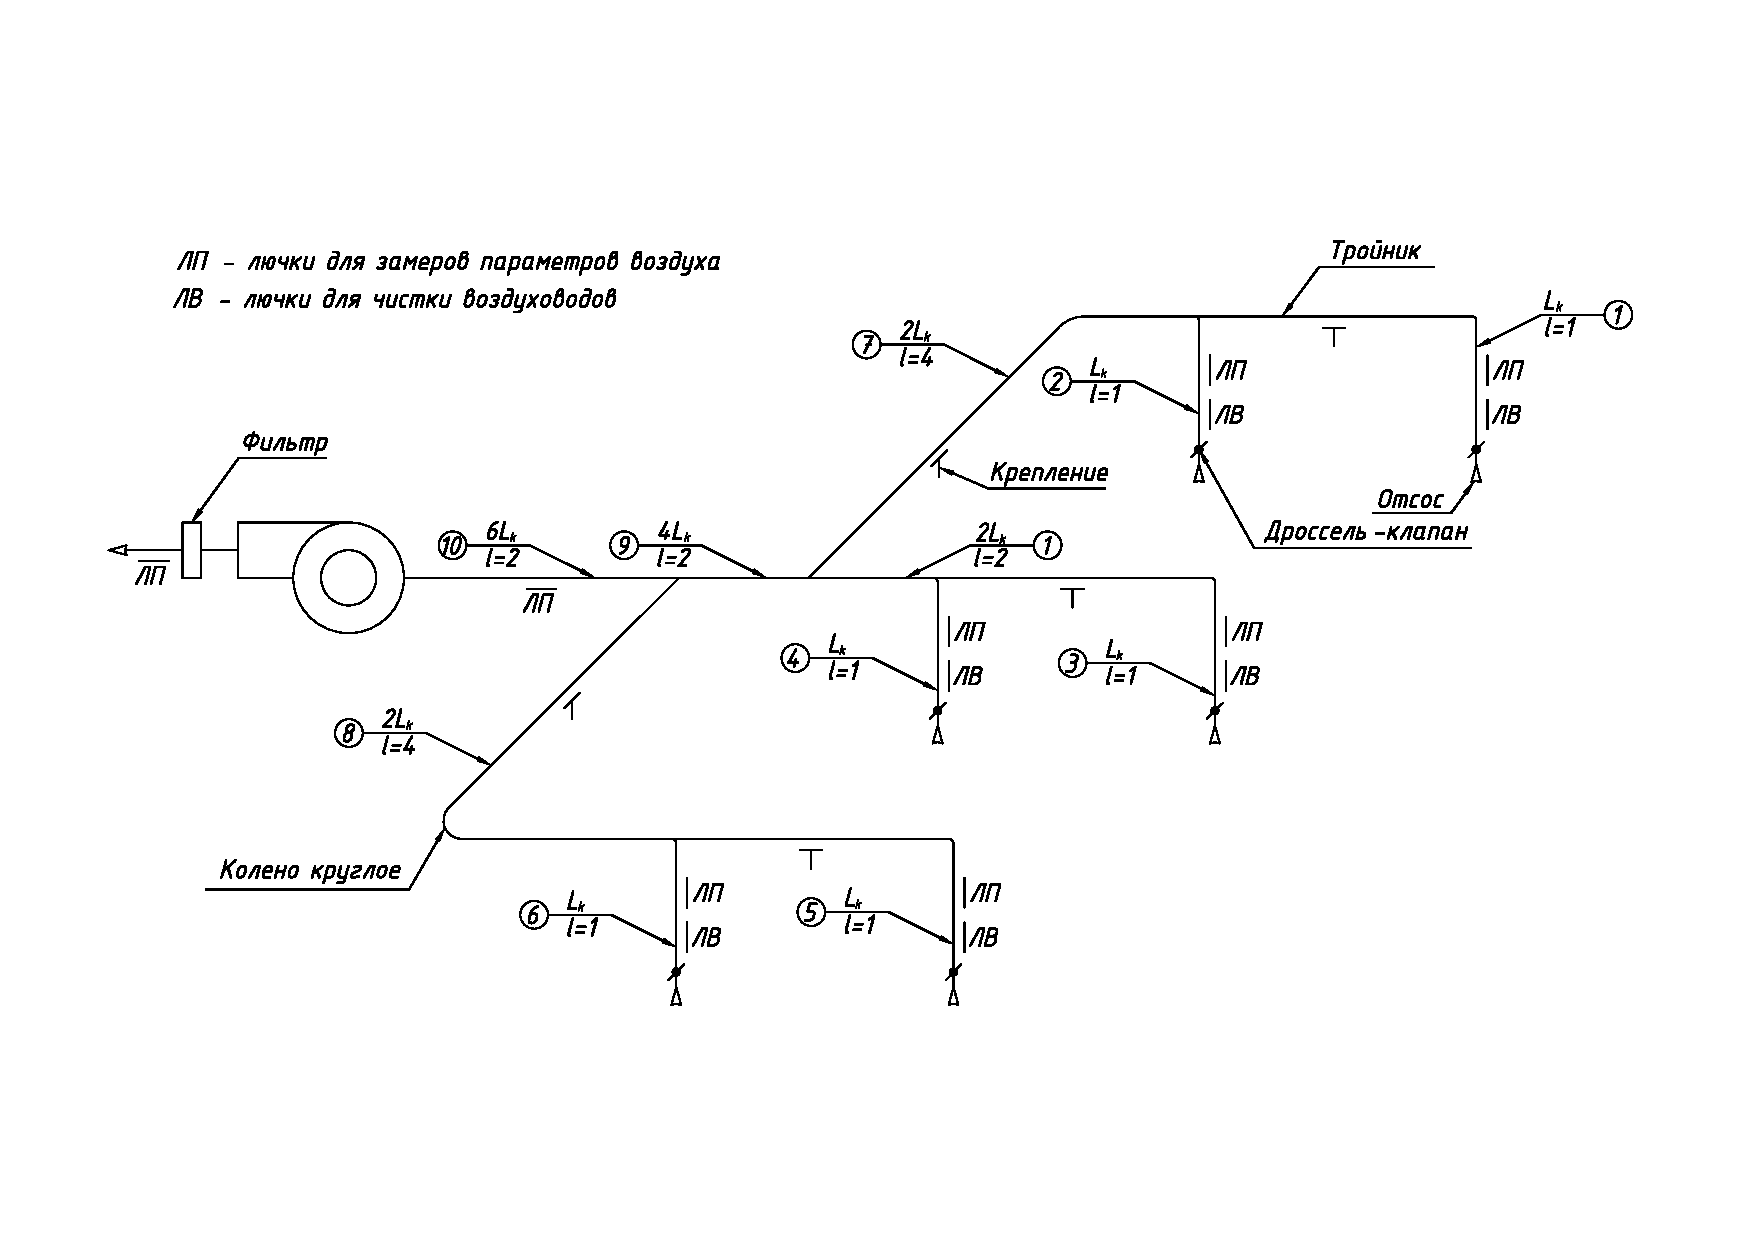
\includegraphics[width=\textwidth, keepaspectratio, clip=true, trim=0mm 35mm 0mm 40mm]
                    {./src/ecology/pictures/vent_system_arrangement}
    \caption{Расчётная схема системы вентиляции}
    \label{pic_vent_system_arrangement}
\end{figure}


\begin{table}
    \centering
    \begin{tabular}{|l|r|r|r|r|r|r|r|r|r|r|}
    \hline
        № уч-ка & L, $\text{м}^3/\text{ч}$  & \textit{l}, мм & d, мм                & V, $\text{м/c}$
        & R, $\text{Н/м}^2$                 & R $\cdot$ \textit{l}, $\text{Н/м}$    & $\sum \rho$
        & $V_{\rho}^2 / 2g, \text{ Н/м}^2$  & $Z, \text{ Н/м}^2$                    & P                 \\
    \hline


    \end{tabular}
    \caption{Основные показатели при расчёте потерь давления в вентиляции}
    \label{pressure_drop_calc_parameters}
\end{table}

Рассчитаем следующие параметры для каждого участка в соотвтетствии со схемой на
рисунке (\ref{pic_vent_system_arrangement}):

\begin{enumerate}
    \item   Расход воздуха \\
            \begin{tabular}{lllll}
                уч-ки 1 - 6:    & $L_k $    & = $f_\text{ж} \cdot V_\text{п}$   & = 1944    & $\text{м}^3 / \text{ч}$ \\
                уч-ки 7 - 9:    & $L_{7-9}$ & = $2 L_k$                         & = 3888    & $\text{м}^3 / \text{ч}$ \\
                уч-к 10:        & $L_{10}$  & = $L_{7} + L_{8}$                 & = 7776    & $\text{м}^3 / \text{ч}$ \\
                уч-к 11:        & $L_{11}$  & = $L_{9} + L_{10}$                & = 11664   & $\text{м}^3 / \text{ч}$ \\
            \end{tabular}

    \item   Длины участков \\
            \begin{tabular}{llll}
                уч-ки 1 - 6:        & $l$           &           & = 1 м \\
                уч-ки 7 и 9:        & $l_{7,9}$     & = $4 l$   & = 4 м \\
                уч-ки 8, 10 и 11:   & $l_{8,10,11}$ & = $2 l$   & = 2 м \\
            \end{tabular}

    \item   Площади и диаметры участков \\
            Воспользуемся формулой, производной от формулы (\ref{air_volume_to_vent})
            для вычисления площади $F_i$ и следующей формулой для вычисления диаметра:
            $$
                d_i = \frac{4}{\pi} \sqrt{F_i}
            $$
            Скорость движения воздуха $V_i$ будем принимать тем большей, чем больше
            расход воздуха в секции.
            \begin{tabular}{lllllllll}
                уч-ки 1 - 6:    & $F_{1-6}$ & = 0,108   & $\text{м}^2$; & $d_{1-6}$ & = 0,37 м; & $V_{1-6}$ & = 5   & $\text{ м/с}$;  \\
                уч-к 7-9:       & $F_{7-9}$ & = 0,166   & $\text{м}^2$; & $d_{7-9}$ & = 0,46 м; & $V_{7-9}$   & = 6,5 & $\text{ м/с}$;  \\
                уч-к 10:        & $F_{10}$  & = 0,2     & $\text{м}^2$; & $d_{10}$  & = 0,51 м; & $V_{10}$  & = 8   & $\text{ м/с}$;  \\
                уч-к 11:        & $F_{11}$  & = 0,25    & $\text{м}^2$; & $d_{11}$  & = 0,56 м; & $V_{11}$  & = 14  & $\text{ м/с}$;  \\
            \end{tabular}

    \item   Потери давления на каждом участке
        \begin{itemize}
            \item   \textbf{Участки 1 - 6} \\
                    Определим потери давления на трение. Потеря давления на единицу длины $R$ по
                    номограмме потери давления в воздуховодах равна
                    $$
                        R_{1-6} = 0,8 \text{ }\frac{\text{Па}}{\text{м}}
                    $$
                    Потеря давления на трение на всём участке
                    $$
                        R_{1-6} \cdot l_{1-6} = 0,8 \text{ Па}
                    $$

                    Местные сопротивления создают: воздухоприёмная панель, дроссель-клапан, колено круглое.
                    Определим их коэффициенты сопротивления:

                    - для неподвижной жалюзийной решетки по
                    \cite{air_ventilation_and_conditioning}[табл. 22.22]
                    $$
                        \xi_\text{ж} = 2
                    $$

                    - для дросселя-клапана при угле открытия $\phi = 15 \degree$ по
                    \cite{air_ventilation_and_conditioning}[табл. 22.33]
                    $$
                        \xi_\text{дк} = 0,9
                    $$

                    - для круглого колена при угле поворота потока в $90 \degree$ и приняв соотношение диаметра отсека к радиусу колена $\frac{d}{r} = 2$ по
                    \cite{air_ventilation_and_conditioning}[табл. 22.26]
                    $$
                        \xi_\text{к} = 0,131 + 0,16 \cdot \left( \frac{d}{r} \right)^{3,5} = 0,15
                    $$

                    Тогда суммарные потери давления:
                    $$
                        P_{1-6} = R_{1-6} \cdot l_{1-6} + \xi_\text{ж} \frac{V_\text{п}^2 \cdot 1,18}{2}
                                    + (\xi_\text{к} + \xi_\text{дк}) \cdot \frac{V_{1-6}^2 \cdot 1,18}{2}
                                = 26,9 \text{ Па}
                    $$

            \item   \textbf{Участки 7 и 9} \\
                    $$
                        R_{7,9} = 1 \text{ }\frac{\text{Па}}{\text{м}}
                    $$
                    $$
                        R_{7,9} \cdot l_{7,9} = 4 \text{ Па}
                    $$

                    Местные сопротивления создают вытяжной тройник и круглое колено.
                    Геометрия тройника определяется площадью трёх сечений его воздуховодов:
                    $F_\text{вх1} = F_{1-6}$ - первое входное сечение,
                    $F_\text{вх2} = F_{1-6}$ - второй входное сечение,
                    $F_\text{вых} = F_{7,9}$ - выходное сечение.

                    Для случая $F_\text{вх1} = F_\text{вх2} = F_\text{вх}$,
                    $F_\text{вх} / F_\text{вых} = 0,6$ и угла между воздуховодами
                    в $90 \degree$ коэффициент сопротивления
                    тройника равен $\xi_\text{тр} = 2$ по
                    \cite{air_ventilation_and_conditioning}[табл. 22.28].

                    Тогда суммарные потери давления:
                    $$
                        P_{1-6} = R_{7,9} \cdot l_{7,9}
                                    + (\xi_\text{тр} + \xi_\text{к}) \cdot \frac{V_{7-9}^2 \cdot 1,18}{2}
                                = 57,9 \text{ Па}
                    $$

            \item   \textbf{Участок 8}
                    $$
                        R_{8} = 1 \text{ }\frac{\text{Па}}{\text{м}}
                    $$
                    $$
                        R_{8} \cdot l_{8,10,11} = 2 \text{ Па}
                    $$

                    Местные сопротивления создаёт только вытяжной тройник.

                    Тогда суммарные потери давления:
                    $$
                        P_{8} = R_{8} \cdot l_{8,10,11}
                                    + \xi_\text{тр} \cdot \frac{V_{7-9}^2 \cdot 1,18}{2}
                                = 51,86 \text{ Па}
                    $$

            \item   \textbf{Участок 10}
                    $$
                        R_{10} = 1,2 \text{ }\frac{\text{Па}}{\text{м}}
                    $$
                    $$
                        R_{10} \cdot l_{8,10,11} = 2,4 \text{ Па}
                    $$

                    Местные сопротивления создаёт вытяжной тройник с коэффициентом
                    сопротивления $\xi_\text{тр.больш} = 2,4$.

                    Тогда суммарные потери давления:
                    $$
                        P_{10} = R_{10} \cdot l_{8,10,11}
                                    + \xi_\text{тр.больш} \cdot \frac{V_{10}^2 \cdot 1,18}{2}
                                = 93 \text{ Па}
                    $$
            \item   \textbf{Участок 11}
                    $$
                        R_{11} = 1,4 \text{ }\frac{\text{Па}}{\text{м}}
                    $$
                    $$
                        R_{11} \cdot l_{8,10,11} = 2,8 \text{ Па}
                    $$

                    Тогда суммарные потери давления:
                    $$
                        P_{11} = R_{11} \cdot l_{8,10,11}
                                    + \xi_\text{тр.больш} \cdot \frac{V_{11}^2 \cdot 1,18}{2}
                                = 280,3 \text{ Па}
                    $$
        \end{itemize}

        \item   Полная потеря давления без учета потерь \\ давления в месте подсоединения вентилятора
                $$
                    P_\text{полн} = 6 \cdot P_{1-6} + 2 \cdot P_{7,9} + P_{8} + P_{10} + P_{11}
                                = 702,36 \text{ Па}
                $$

                Так как транспортируемый воздух загрязнен, то необходимый напор
                определяется по следующей формуле:
                $$
                    P_s = 1,1 \cdot P_\text{полн} = 772,56 \text{ Па}
                $$
\end{enumerate}

\subsubsection{Выбор оборудования}

\paragraph{Вентилятор}
По полученным значениям общей производительности $L_s = 12,83 \cdot 10^3 \text{ м}^3 / \text{ч}$
и давлением $P_s = 772,56 \text{ Па}$ выберем центробежный
вентилятор ВЦ 14-46 из каталога компании «БПО» с частотой вращени
$n = 730 \text{ об/мин}$, производительностью $13,0 \cdot 10^3 \text{ м}^3 / \text{ч}$
и полным давлением 980 Па.

Вентилятор оборудован двигателем АИР132М8 мощность 5,5 кВт.

\paragraph{Фильтр}
Для проектируемой системы выбираем волокнистый ячейковый фильтр.

Максимальная концентрация пыли в рабочей зоне $z_\text{раб.зона} = 0,5 \text{ мг/м}^3$.
Содержание пыли в наружном воздухе непромышленного города $z_\text{город} = 0,6 \text{ мг/м}^3$.

Требуемя эффективность очистки приточного воздуха:

$$
    E_\text{тр} = \frac{z_\text{город} - z_\text{раб.зона}}{z_\text{город}} \cdot 100 \% = 17 \%
$$

Данная степень очистки соответствует классу фильтра тонкой очистки F5, предел эффективности - 60\%
по ГОСТ Р 51251-99 \cite{ecology_gost_51251_99}.
Подберем фильтр по данным \cite{air_ventilation_and_conditioning}[прилож. IV, табл. IV.1]:

\begin{table}[ht]
    \centering
    \begin{tabular}{l|l}
        \hline
        Тип фильтра                                         & волокнистый, замасляный ячейковый ФяУБ            \\
        Фильтрующий материал                                & стекловолокно ФСВУ                                \\
        Номинальная воздушная нагрузка на входное сечение   & $q = 7000 \text{ м}^3/(\text{ч} \cdot \text{м}^2)$\\
        Площадь ячейки                                      & $f_\text{я} = 0,22 \text{м}^2 $                   \\
        Начальное сопротивление                             & $P_\text{ф.н} = 40 \text{ Па}$                    \\
        Конечное сопротивление                              & $P_\text{ф.к} = 150 \text{ Па}$                   \\
        Удельная пылемкость                                 & $\text{П} = 570 \text{ г/м}^2$                    \\
        Способ регенерации                                  & замена фильтрующего материала.                    \\
        \hline
    \end{tabular}
    \caption{Характеристики фильтра}
\end{table}

Требуемая площадь фильтрации в соответствии с формулой (\ref{required_air_exchange}):
$$
    F_\text{ф.тр} = \frac{L}{q} = 1,22 \text{ м}^2
$$

Необходимое количество ячеек:
$$
    n_\text{я} = F_\text{ф.тр} / f_\text{я} = 5,56
                \simeq 6
$$

Действительная степень очистки по номограмме
\cite{air_ventilation_and_conditioning}[прилож. IV, рис. IV.4] $\eta_\text{д} = 84 \%$, что
больше, чем $\eta_\text{тр} = 1 - E_\text{тр} = 83 \%$.

Количество пыли, осаждаемой на $1 \text{ м}^2$ площади фильтрации в течение 1 часа:
$$
    m_\text{уд} = \frac{L \cdot z_\text{город} \cdot \eta_\text{д}}{F_\text{ф.тр}}
            = 1,05 \text{ г/}(\text{м}^2 \cdot \text{ч})
$$

Периодичность замены фильтрующей поверхности:
$$
    \tau_\text{зам} = \text{П} / m_\text{уд} = 23 \text{ сут}
$$

Данная вытяжная система позволяет удалять из воздуха на рабочем месте вредные
вещества до содержания их в пределах допустимой концентрации. Правильная эксплуатация
системы предусматривает периодическое обследование состояния воздушной среды и
элементов вентиляционных установок, а также их правильное обслуживание, своевременную
очистку фильтров воздуховодов, проведение планового ремонта.
